\documentclass{article}

\usepackage{fancyhdr}
\usepackage{extramarks}
\usepackage{amsmath}
\usepackage{amsthm}
\usepackage{amsfonts}
\usepackage{tikz}
\usepackage[plain]{algorithm}
\usepackage{algpseudocode}
\usepackage{enumerate}
\usepackage{amssymb}

\usetikzlibrary{automata,positioning}

%
% Basic Document Settings
%

\topmargin=-0.45in
\evensidemargin=0in
\oddsidemargin=0in
\textwidth=6.5in
\textheight=9.0in
\headsep=0.25in

\linespread{1.1}

\pagestyle{fancy}
\lhead{\hmwkAuthorName}
\chead{\hmwkClass\ (\hmwkClassInstructor\ \hmwkClassTime): \hmwkTitle}
\rhead{\firstxmark}
\lfoot{\lastxmark}
\cfoot{\thepage}

\renewcommand\headrulewidth{0.4pt}
\renewcommand\footrulewidth{0.4pt}

\setlength\parindent{0pt}

%
% Create Problem Sections
%

\newcommand{\enterProblemHeader}[1]{
    \nobreak\extramarks{}{Problem \arabic{#1} continued on next page\ldots}\nobreak{}
    \nobreak\extramarks{Problem \arabic{#1} (continued)}{Problem \arabic{#1} continued on next page\ldots}\nobreak{}
}

\newcommand{\exitProblemHeader}[1]{
    \nobreak\extramarks{Problem \arabic{#1} (continued)}{Problem \arabic{#1} continued on next page\ldots}\nobreak{}
    \stepcounter{#1}
    \nobreak\extramarks{Problem \arabic{#1}}{}\nobreak{}
}

\setcounter{secnumdepth}{0}
\newcounter{partCounter}
\newcounter{homeworkProblemCounter}
\setcounter{homeworkProblemCounter}{1}
\nobreak\extramarks{Problem \arabic{homeworkProblemCounter}}{}\nobreak{}

%
% Homework Problem Environment
%
% This environment takes an optional argument. When given, it will adjust the
% problem counter. This is useful for when the problems given for your
% assignment aren't sequential. See the last 3 problems of this template for an
% example.
%
\newenvironment{homeworkProblem}[1][-1]{
    \ifnum#1>0
        \setcounter{homeworkProblemCounter}{#1}
    \fi
    \section{Problem \arabic{homeworkProblemCounter}}
    \setcounter{partCounter}{1}
    \enterProblemHeader{homeworkProblemCounter}
}{
    \exitProblemHeader{homeworkProblemCounter}
}

%
% Homework Details
%   - Title
%   - Due date
%   - Class
%   - Section/Time
%   - Instructor
%   - Author
%

\newcommand{\hmwkTitle}{Tutorial 9}
\newcommand{\hmwkDueDate}{March 23, 2021}
\newcommand{\hmwkClass}{CZ2003}
\newcommand{\hmwkClassTime}{SS3}
\newcommand{\hmwkClassInstructor}{Assoc Prof Alexei Sourin}
\newcommand{\hmwkAuthorName}{\textbf{Pang Yu Shao}}
\newcommand{\hmwkAuthorID}{\textbf{U1721680D}}

%
% Title Page
%

\title{
    \vspace{2in}
    \textmd{\textbf{\hmwkClass:\ \hmwkTitle}}\\
    \normalsize\vspace{0.1in}\small{Due\ on\ \hmwkDueDate\ at 10:30am}\\
    \vspace{0.1in}\large{\textit{\hmwkClassInstructor\ - \hmwkClassTime}}
    \vspace{3in}\\
    \hmwkAuthorName\\
    \hmwkAuthorID
}

\date{22/03/2021}

\renewcommand{\part}[1]{\textbf{\large Part \Alph{partCounter}}\stepcounter{partCounter}\\}

%
% Various Helper Commands
%

% Useful for algorithms
\newcommand{\alg}[1]{\textsc{\bfseries \footnotesize #1}}

% For derivatives
\newcommand{\deriv}[1]{\frac{\mathrm{d}}{\mathrm{d}x} (#1)}

% For partial derivatives
\newcommand{\pderiv}[2]{\frac{\partial}{\partial #1} (#2)}

% Integral dx
\newcommand{\dx}{\mathrm{d}x}

% Alias for the Solution section header
\newcommand{\solution}{\textbf{\large Solution}}

% Probability commands: Expectation, Variance, Covariance, Bias
\newcommand{\E}{\mathrm{E}}
\newcommand{\Var}{\mathrm{Var}}
\newcommand{\Cov}{\mathrm{Cov}}
\newcommand{\Bias}{\mathrm{Bias}}

\begin{document}

\maketitle

\pagebreak

\begin{homeworkProblem}
   The following VRML code defines a Transform node:\\
   \begin{figure}[H]
      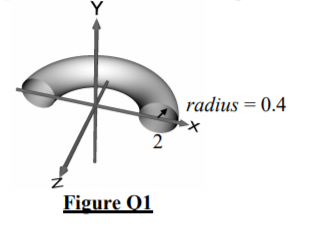
\includegraphics[width=6cm]{fig/q1.PNG}
      \centering
   \end{figure}
   Assuming a column represented position vector, write in a proper order the 
   individual matrices composing this transformation. The final matrix is not required.\\\\
   \textbf{Solution}\\
   Order for VRML Transform node: 1) Scale, 2) Rotation, 3) Translation\\
   \textbf{Scaling}:\\
   $S = \begin{bmatrix}
      3 & 0 & 0 & 0 \\
      0 & 3 & 0 & 0 \\
      0 & 0 & 3 & 0 \\
      0 & 0 & 0 & 1
   \end{bmatrix}$\\\\
   \textbf{Rotation}:\\
   First, Align vector $V=(1, 0 , 1)$ to z-axis
   \begin{figure}[H]
      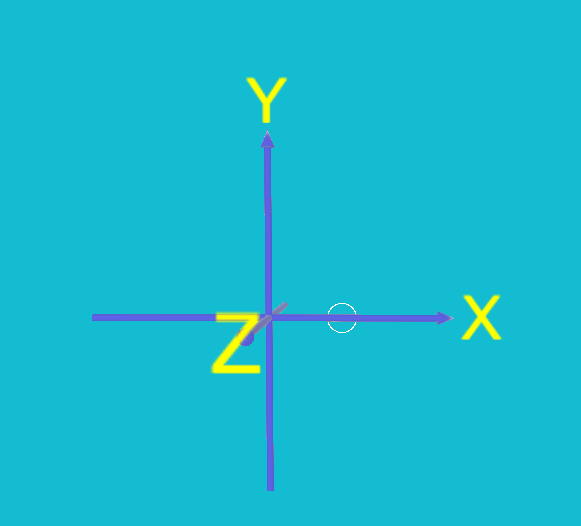
\includegraphics[width=5cm]{fig/q1a.PNG}
      \centering
   \end{figure}
   Angle between V to Z-axis ($\alpha$): \\
   $\alpha = \pi/2 - tan^-1(1)$\\
   $\alpha = \pi/4$\\
   Therefore, first rotate about y-axis by $-\alpha = -\pi/4$\\
   Then, since the rotation axis is aligned with z-axis, rotate about z-axis by $\pi$\\
   Finally, undo the first preprocessing step by rotating about y-axis by $\pi/4$\\\\
   $R = \begin{bmatrix}
      cos(\pi/4) & 0 & sin(\pi/4) & 0 \\
      0 & 1 & 0 & 0 \\
      -sin(\pi/4) & 0 & cos(\pi/4) & 0 \\
      0 & 0 & 0 & 1
   \end{bmatrix}\begin{bmatrix}
      cos(\pi) & -sin(\pi) & 0 & 0 \\
      sin(\pi) & cos(\pi) & 0 & 0 \\
      0 & 0 & 1 & 0 \\
      0 & 0 & 0 & 1
   \end{bmatrix}\begin{bmatrix}
      cos(-\pi/4) & 0 & sin(-\pi/4) & 0 \\
      0 & 1 & 0 & 0 \\
      -sin(-\pi/4) & 0 & cos(-\pi/4) & 0 \\
      0 & 0 & 0 & 1
   \end{bmatrix}$\\
   $R = \begin{bmatrix}
      \sqrt{2}/2 & 0 & \sqrt{2}/2 & 0 \\
      0 & 1 & 0 & 0 \\
      -\sqrt{2}/2 & 0 & \sqrt{2}/2 & 0 \\
      0 & 0 & 0 & 1
   \end{bmatrix}\begin{bmatrix}
      -1 & 0 & 0 & 0 \\
      0 & -1 & 0 & 0 \\
      0 & 0 & 1 & 0 \\
      0 & 0 & 0 & 1
   \end{bmatrix}\begin{bmatrix}
      \sqrt{2}/2 & 0 & -\sqrt{2}/2 & 0 \\
      0 & 1 & 0 & 0 \\
      \sqrt{2}/2 & 0 & \sqrt{2}/2 & 0 \\
      0 & 0 & 0 & 1
   \end{bmatrix}$\\\\
   \textbf{Translation}:\\
   $T = \begin{bmatrix}
      1 & 0 & 0 & 3 \\
      0 & 1 & 0 & 2 \\
      0 & 0 & 1 & 1 \\
      0 & 0 & 0 & 1
   \end{bmatrix}$\\\\

   Therefore, final transformation matrix ($M$):\\
   $M = TRS$\\\\
   $M = \begin{bmatrix}
      1 & 0 & 0 & 3 \\
      0 & 1 & 0 & 2 \\
      0 & 0 & 1 & 1 \\
      0 & 0 & 0 & 1
   \end{bmatrix}
   \begin{bmatrix}
      \sqrt{2}/2 & 0 & \sqrt{2}/2 & 0 \\
      0 & 1 & 0 & 0 \\
      -\sqrt{2}/2 & 0 & \sqrt{2}/2 & 0 \\
      0 & 0 & 0 & 1
   \end{bmatrix}\begin{bmatrix}
      -1 & 0 & 0 & 0 \\
      0 & -1 & 0 & 0 \\
      0 & 0 & 1 & 0 \\
      0 & 0 & 0 & 1
   \end{bmatrix}\begin{bmatrix}
      \sqrt{2}/2 & 0 & -\sqrt{2}/2 & 0 \\
      0 & 1 & 0 & 0 \\
      \sqrt{2}/2 & 0 & \sqrt{2}/2 & 0 \\
      0 & 0 & 0 & 1
   \end{bmatrix}
   \begin{bmatrix}
      3 & 0 & 0 & 0 \\
      0 & 3 & 0 & 0 \\
      0 & 0 & 3 & 0 \\
      0 & 0 & 0 & 1
   \end{bmatrix}$

\end{homeworkProblem}
\pagebreak
\begin{homeworkProblem}
   A unit cube with vertices at points (0,0,0), (0,1,0), (1,1,0), (1,0,0), (0,0,1), …,
   (1,0,1) is transformed into a prism with the respective vertices at points (-1,0,0),
   (-1,2,0), (2,0,0), (2,-2,0), (0,0,2), …, (3,-2,2) by an affine transformation matrix.
   Find a single matrix representing this transformation.\\\\
   \textbf{Solution}\\
   1.) Choose 4 non-coplanar points:\\
   Before transformation: (0,0,0), (0,1,0), (1,1,0), (1,0,1)\\
   After transformation: (-1,0,0), (-1,2,0), (2,0,0), (3,-2,2)\\
   Transformation Matrix: $M$
   
   $M = \begin{bmatrix}
         a & b & c & l \\
         d & e & f & m \\
         g & h & i & n \\
         0 & 0 & 0 & 1
      \end{bmatrix}$\\\\
      Therefore,\\\\
      $\begin{bmatrix}
         a & b & c & l \\
         d & e & f & m \\
         g & h & i & n \\
         0 & 0 & 0 & 1
      \end{bmatrix}\begin{bmatrix}
         0 \\
         0 \\
         0 \\
         1
      \end{bmatrix} = \begin{bmatrix}
         -1 \\
         0 \\
         0 \\
         1
      \end{bmatrix}$\\
      $\mathbf{l = -1, m = 0, n = 0}$
      \\\\
      $\begin{bmatrix}
         a & b & c & -1 \\
         d & e & f & 0 \\
         g & h & i & 0 \\
         0 & 0 & 0 & 1
      \end{bmatrix}\begin{bmatrix}
         0 \\
         1 \\
         0 \\
         1
      \end{bmatrix} = \begin{bmatrix}
         -1 \\
         2 \\
         0 \\
         1
      \end{bmatrix}$\\
      $b - 1 = -1$\\ 
      $\mathbf{b = 0}, \mathbf{e = 2}, \mathbf{h = 0}$
      \\\\
      $\begin{bmatrix}
         a & 0 & c & -1 \\
         d & 2 & f & 0 \\
         g & 0 & i & 0 \\
         0 & 0 & 0 & 1
      \end{bmatrix}\begin{bmatrix}
         1 \\
         1 \\
         0 \\
         1
      \end{bmatrix} = \begin{bmatrix}
         2 \\
         0 \\
         0 \\
         1
      \end{bmatrix}$\\
      $(a - 1 = 2),\ (d + 2 = 0),\ (g = 0)$\\
      $\mathbf{a = 3}, \mathbf{d = -2}, \mathbf{g = 0}$\\
      \\\\
      $\begin{bmatrix}
         3 & 0 & c & -1 \\
         -2 & 2 & f & 0 \\
         0 & 0 & i & 0 \\
         0 & 0 & 0 & 1
      \end{bmatrix}\begin{bmatrix}
         1 \\
         0 \\
         1 \\
         1
      \end{bmatrix} = \begin{bmatrix}
         3 \\
         -2 \\
         2 \\
         1
      \end{bmatrix}$\\
      $(3 + c - 1 = 3),\ (-2 + f  = -2),\ (i = 2)$\\
      $\mathbf{c = 1}, \mathbf{f = 0}, \mathbf{i = 2}$\\\\
      $\therefore \mathbf{M = \begin{bmatrix}
         3 & 0 & 1 & -1 \\
         -2 & 2 & 0 & 0 \\
         0 & 0 & 2 & 0 \\
         0 & 0 & 0 & 1
      \end{bmatrix}}$

    
\end{homeworkProblem}

\pagebreak
\begin{homeworkProblem}
    Assuming a column represented position vector, write in a proper order individual matrices implementing
    the transformation of reflection about a straight line defined parametrically by $x=1-t$, $y=0$, $z=2t$, 
    $t\in(-\infty, \infty)$. The final matrix is not required.\\\\
    \textbf{Solution}\\
    To get straight line, get for t = 1, 0 and -1\\
    t=-1: $(2, 0, -2)$\\
    t=0: $(1, 0, 0)$\\
    t=1: $(0, 0, 2)$\\
    By visualizing the reflection, we get the following figure:
    \begin{figure}[H]
      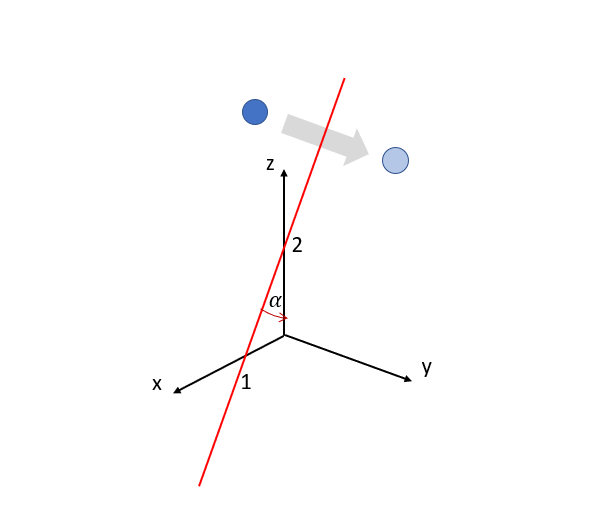
\includegraphics[width=9cm]{fig/q3a.PNG}
      \centering
   \end{figure}

   Where $\alpha = tan^-1(1/2) = 0.463$

   Therefore, the following steps are required:\\
   1) Translate by -1 in x-axis such that the reflection axis passes through the origin\\
   $T_1 = \begin{bmatrix}
      1 & 0 & 0 & -1 \\
      0 & 1 & 0 & 0 \\
      0 & 0 & 1 & 0 \\
      0 & 0 & 0 & 1
   \end{bmatrix}$\\
   2) Rotate about y-axis for an angle of $\alpha$ such that the reflection axis is aligned with z-axis\\
   $R_2 = \begin{bmatrix}
      cos(0.463) & 0 & sin(0.463) & 0 \\
      0 & 1 & 0 & 0 \\
      -sin(0.463) & 0 & cos(0.463) & 0 \\
      0 & 0 & 0 & 1
   \end{bmatrix} = \begin{bmatrix}
      0.894 & 0 & 0.447 & 0 \\
      0 & 1 & 0 & 0 \\
      -0.447 & 0 & 0.894 & 0 \\
      0 & 0 & 0 & 1
   \end{bmatrix}$\\
   3) Perform reflection about z-axis\\
   $R_3 = \begin{bmatrix}
      -1 & 0 & 0 & 0 \\
      0 & -1 & 0 & 0 \\
      0 & 0 & 1 & 0 \\
      0 & 0 & 0 & 1
   \end{bmatrix}$\\
   4) Rotate about y-axis for an angle of $-\alpha$ (undo step 2)\\
   $R_4 = \begin{bmatrix}
      cos(-0.463) & 0 & sin(-0.463) & 0 \\
      0 & 1 & 0 & 0 \\
      -sin(-0.463) & 0 & cos(-0.463) & 0 \\
      0 & 0 & 0 & 1
   \end{bmatrix} = \begin{bmatrix}
      0.894 & 0 & -0.447 & 0 \\
      0 & 1 & 0 & 0 \\
      0.447 & 0 & 0.894 & 0 \\
      0 & 0 & 0 & 1
   \end{bmatrix}$\\
   5) Translate by 1 in x-axis (undo step 1)\\
   $T_5 = \begin{bmatrix}
      1 & 0 & 0 & 1 \\
      0 & 1 & 0 & 0 \\
      0 & 0 & 1 & 0 \\
      0 & 0 & 0 & 1
   \end{bmatrix}$\\\\

   Therefore, final transformation matrix ($M$):\\
   $M = T_5R_4R_3R_2T_1$\\\\
   $M = \begin{bmatrix}
      1 & 0 & 0 & 1 \\
      0 & 1 & 0 & 0 \\
      0 & 0 & 1 & 0 \\
      0 & 0 & 0 & 1
   \end{bmatrix}\begin{bmatrix}
      0.894 & 0 & -0.447 & 0 \\
      0 & 1 & 0 & 0 \\
      0.447 & 0 & 0.894 & 0 \\
      0 & 0 & 0 & 1
   \end{bmatrix}\begin{bmatrix}
      -1 & 0 & 0 & 0 \\
      0 & -1 & 0 & 0 \\
      0 & 0 & 1 & 0 \\
      0 & 0 & 0 & 1
   \end{bmatrix}\begin{bmatrix}
      0.894 & 0 & 0.447 & 0 \\
      0 & 1 & 0 & 0 \\
      -0.447 & 0 & 0.894 & 0 \\
      0 & 0 & 0 & 1
   \end{bmatrix}\begin{bmatrix}
      1 & 0 & 0 & -1 \\
      0 & 1 & 0 & 0 \\
      0 & 0 & 1 & 0 \\
      0 & 0 & 0 & 1
   \end{bmatrix}$\\\\




    


\end{homeworkProblem}

\pagebreak
\begin{homeworkProblem}
   A semi-circle on the ZX plane in shown in Fig.4 (left). It undergoes a sweeping by a full rotation about the 
   Y-axis and a translation along the Y-axis by 2 units simultaneously, which provides a surface shown in Fig.4(right).
   Utilizing transformation matrices. derive a parametric representation of the surface.
    \begin{figure}[H]
      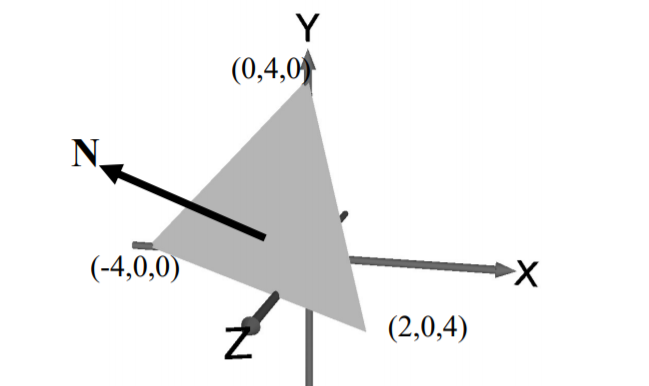
\includegraphics[width=8cm]{fig/q4.PNG}
      \centering
   \end{figure}
   \textbf{Solution}\\
   Step 1: define parametric equations for the semi-circle curve.\\
   \[
      \begin{split}
      x_0(\alpha) &= sin(\alpha)\\
      y_0(\alpha) &= 0\\
      z_0(\alpha) &= 1+cos(\alpha)\\
      &alpha \in [0, \pi]
      \end{split}
   \]
   Step 2: Multiply the coordinates by 3D rotation matrix and figure out range of
   rotation angle\\
   \[
   \begin{split}
      \begin{bmatrix}
         x(\alpha,\beta)\\
         y(\alpha,\beta)\\
         z(\alpha,\beta)\\
         1
      \end{bmatrix}
      &= \begin{bmatrix}
         cos(\beta) & 0 & sin(\beta) & 0 \\
         0 & 1 & 0 & 0 \\
         -sin(\beta) & 0 & cos(\beta) & 0 \\
         0 & 0 & 0 & 1
      \end{bmatrix}\begin{bmatrix}
         x_0(\alpha)\\
         y_0(\alpha)\\
         z_0(\alpha)\\
         1
      \end{bmatrix}
   \end{split}
   \]

   \[
      \begin{split}
      x(\alpha,\beta) &= cos(\beta)x_0(\alpha) + sin(\beta)z_0(\alpha)\\
      y(\alpha,\beta) &= y_0(\alpha)\\
      z(\alpha, \beta) &= -sin(\beta)x_0(\alpha) + cos(\beta)z_0(\alpha)\\
      &\beta\in[0, 2\pi]
      \end{split}
   \]
   Step 3: Handle translational sweeping
   \[
      \begin{split}
      y(\alpha,\beta) &= y_0(\alpha) + f(\beta)\\
      f(\beta) &= A + B\beta\\
      f(0) &= A\\
      &= 0\\
      \therefore A &= 0\\
      f(2\pi) &= 2\pi B\\
      &= 2\\
      \therefore B &= 1/\pi\\\\
      \therefore y(\alpha,\beta) &= y_0(\alpha) + \beta / \pi\\
      \end{split}
   \]
   \[
      \begin{split}
      x(\alpha,\beta) &= cos(\beta)sin(\alpha) + sin(\beta)(1+cos(\alpha))\\
      y(\alpha,\beta) &= \beta / \pi\\
      z(\alpha, \beta) &= -sin(\beta)sin(\alpha) + cos(\beta)(1+cos(\alpha))\\
      &alpha \in [0, \pi]\ \ \beta\in[0, 2\pi]
      \end{split}
   \]
   Step 4: Rename $\alpha, \beta$ to $u,v$, $u,v \in [0,1]$
   \[
      \begin{split}
      u &= \alpha/\pi \\
      v &= \beta/2\pi
      \end{split}
   \]
   Therefore,
   \[
      \begin{split}
      x(u,v) &= cos(2\pi v)sin(\pi u) + sin(2\pi v)(1+cos(\pi u))\\
      y(u,v) &= 2v\\
      z(u,v) &= -sin(2\pi v)sin(\pi u) + cos(2\pi v)(1+cos(\pi u))\\
      &u,v \in [0,1]
      \end{split}
   \]
   \begin{figure}[H]
      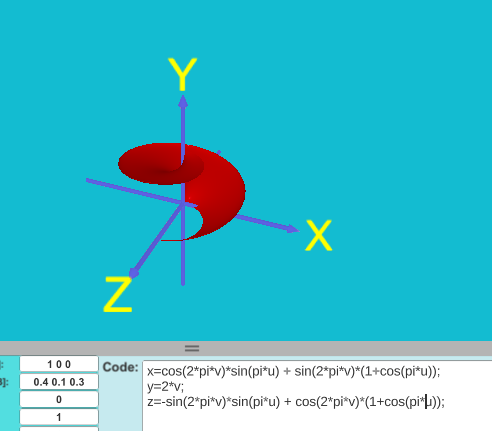
\includegraphics[width=14cm]{fig/q4a.PNG}
      \centering
   \end{figure}
    
\end{homeworkProblem}

\end{document}